\subsection{Relační datový model}
Relační datový model představuje \textbf{způsob uchování dat v tabulkách}. Relační se mu říká proto, jelikož tabulka je definována přes Relaci.

\begin{figure}[H]
	\centering
	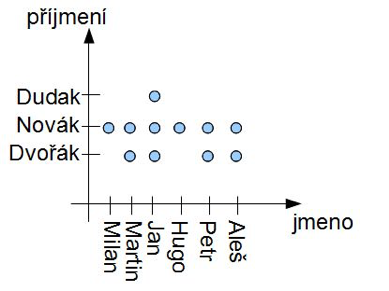
\includegraphics[width=0.35\textwidth]{assets/tab_relace.png}
	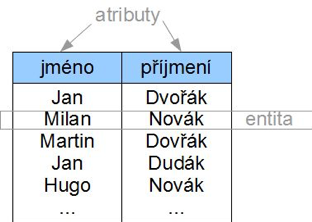
\includegraphics[width=0.35\textwidth]{assets/relace.png}
	\caption{Tabulka s dvěma atributy jako relace (vlevo), relace zobrazena tabulkou (vpravo).}
\end{figure}

\textbf{Relace} je tabulka definována jako \textbf{podmnožina kartézského součinu domén}. Relace na obrázku je tedy podmnožina kartézského součinu množin \{Dudak, Novák, Dvořák\} $\times$ \{Milan, Martin, Jan, ..., Aleš\}.

Na rozdíl od matematické relace se ta databázová \textbf{mění v čase} (přidáváním a odebíráním prvků relace). Kromě základních \textbf{množinových operací} se u databázové relace setkáme s operaci \textbf{selekce} -- výběr řádků a \textbf{projekce} -- výběr sloupců.

\begin{itemize}
\item \textbf{Doména} je \textbf{množina všech hodnot, kterých může daný atribut nabývat} (obor hodnot atributu). V praxi je doména dána\textbf{ integritním omezením} (IO). Doména atributu Přijmení z obrázků je množina \{Dudak, Novák, Dvořák\}.
\item \textbf{Atribut} je vlastnost entity (z pohledu tabulky jde o sloupec).
\item \textbf{Relační schéma} můžeme chápat jako strukturu tabulky (atributy a domény).
Relační schéma R je výraz tvaru R(A, f),  kde  R  je jméno schématu, A = {A1, A2,..., An} je \textbf{konečná množina jmen atributů}, f je zobrazení přiřazující každému jménu atributu Ai neprázdnou množinu (obor hodnot atributu), kterou nazýváme \textbf{doménou atributu} Di, tedy \textbf{f(Ai) = Di}.
\end{itemize}

\subsubsection*{Příklad pro tabulku (relaci) Učitel}
\begin{itemize}
\item \textbf{Atributy:} \texttt{ID, jméno, příjmení, funkce, kancelář}.
\item \textbf{Domény:} 
\begin{itemize}
\item D1 -- tři písmena z příjmení, tří cifry pořadového čísla,
\item D2 -- kalendář jmen,
\item D3 -- množina příjmení,
\item D4 -- množina funkcí (asistent, vědec, učitel,...),
\item D5 -- A101, A102, ... A160.
\end{itemize}
\item \textbf{Relační schéma:} \texttt{Učitel (ID, jméno, příjmení, funkce, kancelář)}.
\item \textbf{Relace:} \texttt{Učitel = \{(nov001, lukas , novak , vědec, A135),\\ (kom123, jan, komensky, učitel, A111), ...\}}
\end{itemize}

\subsubsection{Základní úlohy relačního modelu:}
\begin{enumerate}
\item Návrh „správné“ \textbf{struktury databáze bez redundancí} -- \textbf{funkční závislosti}, \textbf{normální formy}.
\item \textbf{Vyhledávání informací} z databáze -- (dotazovací) \textbf{relační jazyky}.
\end{enumerate}

\subsubsection{Vlastnosti relačního datového modelu}
Z definice relace vyplývají tyto jejich tabulkové vlastnosti:
\begin{itemize}
\item \textbf{Homogenita} (stejnorodost) sloupců (prvky domény).
\item Každý údaj (hodnota atributu ve sloupci) je \textbf{atomickou položkou}.
\item Na \textbf{pořadí} řádků a sloupců \textbf{nezáleží} (jsou to množiny prvků/atributů).
\item Každý řádek tabulky je \textbf{jednoznačně identifikovatelný} hodnotami jednoho nebo několika atributů (primárního klíče).
\end{itemize}

\subsubsection{Vazby relačního modelu}
Obecně se vazby v relačním modelu realizují pomocí další relace (tabulky). Jedná se o tzv. \textbf{vazební tabulku}. Ta obsahuje ty atributy relací (tabulek, které se vazby účastní), které jednoznačné identifikují jejich entity -- primární klíče. Obsahuje-li tabulka atribut, který slouží jako primární klíč v jiné tabulce, pak obsahuje cizí klíč. Vazební tabulka tedy obsahuje cizí klíče. Příklad vazby M:N:

\begin{figure}[H]
	\centering
	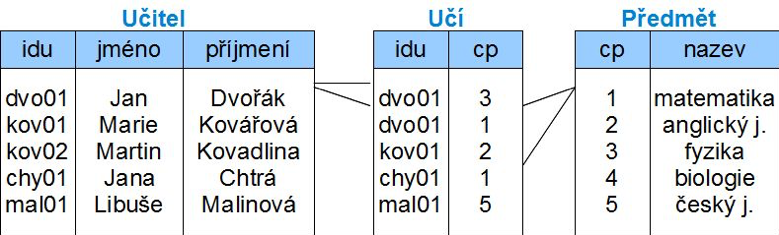
\includegraphics[width=0.8\textwidth]{assets/mn.png}
\end{figure}

\subsection{SQL (Structured Query Language)}
SQL (Structured Query Language) \textbf{je relační jazyk založen na predikátovém kalkulu}. Na rozdíl od jazyků založených na relační algebře, kde se dotaz zadává algoritmem, tyto jazyky se soustředí na to \textbf{co se má hledat}, ne jak.

\begin{itemize}
	\item Standardizovaný\textbf{ strukturovaný dotazovací jazyk}, který je používán pro práci s daty v \textbf{relačních databázích}. (DQL - Data Query Language).
	\item Navržen IBM jako \textbf{dotazovací jazyk} (původní název Sequel).
	\item Základem je \textbf{n-ticový relační kalkul}.
	\item Standardy podporuje prakticky každá relační databáze, ale obvykle nejsou implementovány vždy\textbf{ všechny požadavky normy}.
	\item Obsahuje i příkazy pro \textbf{vytvoření} a \textbf{modifikace} tabulek, pro \textbf{ukládání}, \textbf{modifikaci} a \textbf{rušení} dat v databázi a řadu dalších příkazů.
	\item \textbf{Příklad}: \texttt{CREATE TABLE Drazitel (jmeno CHAR(20), adresa CHAR(30), aukce NUMBER(4), zisk NUMBER(4)); INSERT INTO  clovek VALUES( 'nj001', 'Jan', 'Novotný', '777111222'); SELECT telefon FROM clovek WHERE prijmeni = "Novotný";}
\end{itemize}

\subsubsection{DML - Data manipulation language}
\begin{itemize}
	\item \textbf{Modifikací} dat --  \texttt{INSERT}, \texttt{UPDATE}, \texttt{DELETE} = vlož, uprav, smaž.
	\item \textbf{Vyhledávání} v relacích --  \texttt{SELECT}, \texttt{ORDER BY},  \texttt{GROUP BY}, \texttt{JOIN} = vyhledej, seřaď, shlukuj, spoj.	
	\item Další, pro podmínky, logické operatory, ... (\texttt{WHERE, LIKE, BETWEEN, IN, IS NULL, DISTINCT/UNIQUE, JOIN, INNER JOIN, OUTER JOIN, EXISTS, HAVING, COUNT, VIEW, INDEX}, ...).
\end{itemize}

\subsubsection{DDL - Data definition language}
\begin{itemize}
	\item \textbf{Vytváření} a \textbf{modifikace} relačního schematu (tabulek, databází) - \texttt{CREATE}, \texttt{ALTER} (\texttt{MODIFY}, \texttt{ADD}), \texttt{DROP}  = vytvoř, uprav, smaž.
\end{itemize}

\subsubsection{DCL - Data control language}
\begin{itemize}
	\item \textbf{Správa práv} - příkazy jako \texttt{GRANT}, \texttt{REVOKE}.
\end{itemize}

\subsubsection{TCL - Transaction control language - transakce}
\begin{itemize}
	\item \texttt{COMMIT} - úspěšně provedená transakce, vše se uloží.
	\item \texttt{ROLLBACK} - zrušení všech změn celé transakce.
	\item \texttt{SAVEPOINT} - uložení bodu, ke kterému lze provést \texttt{ROLLBACK}. Tj zruší se jen část transakce a může se pokračovat jinou větví celé transakce dále. Lze tak transakce dělit na menší atomické části.
\end{itemize}

\subsection{Relační jazyky}
Jazyky pro formulaci požadavků na výběr dat z relační databáze (dotazovací jazyky) se dělí do dvou skupin:
\begin{itemize}
\item \textbf{Jazyky založené na  relační algebře}, kde jsou výběrové požadavky vyjádřeny jako posloupnost speciálních operací prováděných nad daty. Dotaz je tedy  \textbf{zadán algoritmem}, jak vyhledat požadované informace.
\item \textbf{Jazyky založené na  predikátovém kalkulu}, které požadavky na výběr zadávají jako predikát charakterizující \textbf{vybranou relaci}. Je úlohou překladače jazyka nalézt odpovídající algoritmus. Tyto jazyky se dále dělí na 
\begin{itemize}
	\item \textbf{n-ticové} relační kalkuly,
	\item \textbf{doménové} relační kalkuly. 
\end{itemize}
\end{itemize}

\subsection{Relační algebra}
Relační algebra je velmi silný \textbf{dotazovací jazyk} vysoké úrovně. Nepracuje s jednotlivými enticemi relací, ale \textbf{s celými relacemi}. Operátory relační algebry se aplikují na relace, výsledkem jsou opět relace. Protože relace jsou množiny, přirozenými prostředky pro manipulaci s relacemi budou množinové operace.

I když relační algebra v této podobě \textbf{není vždy implementována v jazycích SŘBD}, je její zvládnutí nutnou podmínkou pro správnost manipulací s relacemi. I složitější dotazy jazyka SQL, který je deskriptivním dotazovacím jazykem, mohou být bez zkušeností s relační algebrou problematické. 

\subsubsection{Základní operace relační algebry}
Jsou dány relace \textbf{R} a \textbf{S}. \textbf{Množinové operace:}
\begin{itemize}
\item \textbf{Sjednocení} relací téhož stupně:      $R \cup S = \{x | x \in R \vee x \in S\}$
\item \textbf{Průnik} relací:                                 $R \cap S = \{x | x \in R \wedge x \in S\}$
\item \textbf{Rozdíl} relací:                                   $R  -  S = \{x | x \in R \wedge x \notin S\}$
\item \textbf{Kartézský součin} relace R stupně m a relace S stupně n: $R x S = \{rs | r \in R \wedge s \in S\}$,  kde  $rs = \{r1,...,rm,s1,...sn\}$
\end{itemize}
\textbf{Další relační operace: }
\begin{itemize}
\item \textbf{Projekce} (výběr atributů) relace R, jedná se o unární operaci $\Pi_\mathbf{X}( R )$, kde X je množina názvů atributů.
\item \textbf{Selekce} (výběr řádků) z relace R podle podmínky P. Selekce je unární relační operace $\sigma_{\varphi(\mathbf{X})}( R )$, kde R je relace, $\varphi(\mathbf{X})$ predikátová formule hovořící o jednotlivých prvcích a jejich příslušnosti do relací.
\item \textbf{Spojení} relací R s atributy A  a  S  s atributy  B (join).  Značí se $R \bowtie S$, výsledkem je množina všech kombinací prvků relace \textbf{R} a \textbf{S}. Takto definovaný join se nazývá Přirozené spojení (natural join). Exsitují i další (outer, inner, left, right \ldots).
\end{itemize}

Příklad: $\Pi_\textrm{název} \sigma_{\varphi(\textrm{pohlaví=žena})} (\textrm{Úkol}\bowtie\textrm{Pracuje}\bowtie\textrm{Zaměstnanec})$


\subsection{N-ticový relační kalkul}
\begin{itemize}
\item Dr. Codd definoval n-ticový relační kalkul pro RDM jazyk matematické logiky - predikátový počet je využit pro výběr informací z relační databáze.
\item Název odvozen z oboru hodnot jeho proměnných - \textbf{relace je množina prvků = n-tic}.
\item Je \textbf{základem pro jazyk typu SQL}.
\item Syntaxe je \textbf{přizpůsobena} programovacímu jazyku: \textbf{matematické vyjádření} $\{ x | F(x) \}$ nahradíme zápisem \textbf{\texttt{x WHERE  F(x)}}
\begin{itemize}
\item Kde x je proměnná pro hledané n-tice (struktura relace).
\item F(x) je \textbf{podmínka}, kterou má x splňovat (výběr prvků relace).
\end{itemize}
\end{itemize}

\subsubsection{Definice}
Výraz n-ticového relačního kalkulu je výraz tvaru \textbf{\texttt{x WHERE F(x)}}, kde x je jediná volná proměnná ve formuli F. Základní operace relační algebry se dají vyjádřit pomocí výrazů n-ticového relačního kalkulu, tedy n-ticový relační kalkul je relačně úplný.

\noindent\makebox[\textwidth]{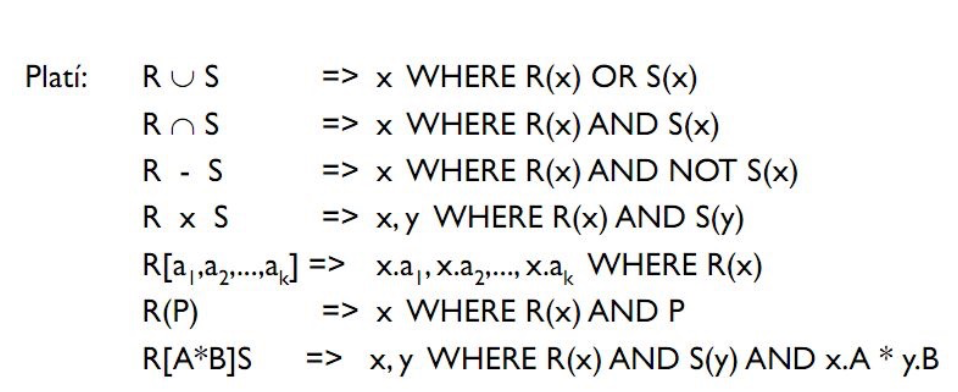
\includegraphics[width=12cm]{assets/ntic}}


\subsection{Funkční závislost}
Funkční závislost je v databázi \textbf{vztah mezi atributy} takový, že máme-li atribut Y je funkčně závislý na atributu X píšeme X → Y, pak se \textbf{nemůže stát}, aby \textbf{dva řádky mající stejnou} hodnotu atributu \textbf{X} měly \textbf{různou hodnotu Y}. Je-li Y, X říkáme, že závislost X → Y je \textbf{triviální}.
\begin{itemize}
\item FZ je definována \textbf{mezi dvěma podmnožinami atributů} v rámci jednoho schématu relace. Jde o vztah mezi atributy, nikoliv mezi entitami.
\item FZ je definována na \textbf{základě všech možných aktuálních relací}, není tedy možné soudit na funkční závislost z vlastností jediné relace. Tak můžeme poznat jen neplatnost funkční závislosti.
\item FZ jsou \textbf{tvrzení o reálném světě}, o významu atributů nebo \textbf{vztahů mezi entitami}, je nutné realitu brát v úvahu při návrhu schématu databáze.
\end{itemize}

\textbf{Příklad:} Atribut '\textit{datum narození }' je funkčně závislý na atributu '\textit{rodné číslo}' (nemůže se stát, že u záznamů se stejnými rodnými čísly bude různé datum narození).

Pomocí funkčních závislostí můžeme\textbf{ automaticky navrhnout schéma databáze} a předejít problémům jako je \textbf{redundance}, \textbf{nekonzistence databáze}, zablokování při vkládání záznamů, apod.

\subsection{Armstrongovy axiomy}
K určení \textbf{klíče schématu} a logických implikací množiny závislostí potřebujeme \textbf{nalézt uzávěr F+}, nebo určit, zda daná závislost X → Y je prvkem F+.  K tomu existují pravidla zvaná Armstrongovy axiomy. Jsou \textbf{úplná} (dovolují odvodit z dané množiny závislostí F všechny závislosti patřící do F+) a \textbf{bezesporná} (dovolují z F odvodit pouze závislosti patřící do F+).
\begin{itemize}
\item \textbf{Reflexivita} -- je-li Y $\subset$ X $\subset$ A, pak X → Y
\item \textbf{Tranzitivita} -- pokud je X → Y a Y → Z, pak X → Z
\item \textbf{Pseudotranzitivita} --  pokud je X → Y a WY → Z, pak XW → Z
\item \textbf{Sjednocení} -- pokud je X → Y a X → Z, pak X  → YZ
\item \textbf{Dekompozice} -- pokud je X → YZ, pak  X  → Y a X → Z
\item \textbf{Rozšíření} --  pokud je X → Y a  Z $\subset$ A, pak  XZ  → YZ
\item \textbf{Zúžení} --  pokud je X → Y a  Z  $\subset$ Y, pak  X → Z
\end{itemize}
Závislost, která má na pravé straně pouze jeden atribut, nazýváme \textbf{elementární}. 

\subsubsection{Určení klíče pomoci funkčních závislostí}
Ze zadání jsme určili atributy A = \{učitel, jméno, příjmení, email, předmět, název, kredity, místnost, čas\} a funkční závislosti F:
\begin{itemize}
	\item učitel → jméno, příjmení, email
	\item předmět → název, kredity
	\item místnost, čas → učitel, předmět
\end{itemize}

\noindent\textbf{Rozšíření:}
\begin{itemize}
\item učitel, \textbf{místnost}, \textbf{čas} → jméno, příjmení, email, \textbf{místnost}, \textbf{čas}
\item předmět → název, kredity
\item místnost, čas → učitel, předmět
\end{itemize}

\noindent\textbf{Dekompozice 1:}
\begin{itemize}
\item učitel, \textbf{místnost}, \textbf{čas} → jméno, příjmení, email, místnost, čas, \textbf{učitel}, \textbf{předmět}
\item předmět → název, kredity
\end{itemize}

\noindent\textbf{Dekompozice 2:}
\begin{itemize}
\item učitel, místnost, čas → jméno, příjmení, email, místnost, čas, učitel, předmět, \textbf{název}, \textbf{kredity}
\end{itemize}

Atributy \textbf{učitel}, \textbf{místnost}, \textbf{čas} je klíč schématu velké relace. V dalším kroku je třeba provést dekompozici a tuto velkou relaci rozbít na menší relace.

\subsection{Dekompozice}
Dekompozice relačního schématu je \textbf{rozklad relačního schématu na menší} relač. sch. (rozloží velkou tabulku na menší) aniž by došlo k narušení redundance databáze. Mezi základní vlastnosti dekompozice patří - \textbf{zachování informace} a \textbf{zachování funkčních závislostí}.
\begin{itemize}
\item \textbf{Algoritmus dekompozice (metoda shora dolů)} -- na počátku máme celé relační schéma se všemi atributy, snažíme se od tohoto schématu odebírat funkční závislosti a tvořit schémata nová. \textbf{Exponenciální složitost}, \textbf{BCNF}.
\item \textbf{Algoritmus syntézy (zdola nahoru)} -- vytvoří pro každou funkční závislost novou relaci. Pak tyto malé relace spojuje do větších celků. \textbf{Menší složitost, 3NF}.
\end{itemize}
\textbf{Binární dekompozice}, kterou budeme dále řešit je rozklad jednoho relačního schématu na dvě. Obecná dekompozice vznikne postupnou aplikací binárních. Dekompozice relačního schématu R(A,f) je množina relačních RO=\{R1(A1, f2), R2(A2, f2), ...\}, kde A = A1 $\cup$ A2 $\cup$ A3 $\cup$ ...

\subsection{Normální formy}
Normální formy relací (NF) prozrazují jak dobře je databáze navržena (čím vyšší NF tím lepší).
\begin{itemize}
\item \textbf{0 NF} -- Pokud nesplňuje ani 1 NF, je v 0 NF
\item \textbf{1 NF} -- definuje tabulky, které obsahují \textbf{pouze atomické atributy}. Žádné složené atributy - např. v jednom atributu je Jméno i Příjmení.
\item \textbf{2 NF} -- je v 1NF + \textbf{každý sekundární atribut je úplně závislý na každém klíči schématu}. Neboli neexistuje závislost sekundárních na podklíči (pokud se klíč skládá z více atributů). Např.: když AB → CD, pak nesmí být B → C. Atribut adresa není závislý na všech klíčích FZ, ale pouze na F.
\begin{figure}[H]
	\centering
	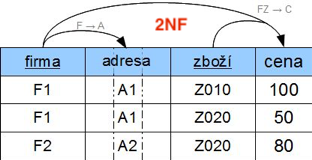
\includegraphics[width=0.4\textwidth]{assets/2nf.png}
\end{figure}
\item \textbf{3 NF} -- je 2NF + žádný sekundární atribut \textbf{není tranzitivně závislý} na žádném klíči schématu. Nesmí existovat závislosti mezi sekundárními atributy (Model auta -> značka auta). Když AB → CD, pak nesmí C  → D. \textbf{Příklad porušení 3NF} -- atribut počet obyvatel je tranzitivně závislý (přes atr. město) na klíči.
\begin{figure}[H]
	\centering
	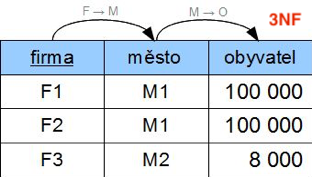
\includegraphics[width=0.4\textwidth]{assets/3nf.png}
\end{figure}
\item \textbf{BCNF} (Boyce-Coddova normální forma) -- 3NF + je-li funkční závislost (X → Y) $\in$ F+ a Y $\notin$ X, pak X obsahuje klíč schématu. \textbf{Musí být závislost sekundárních atributů na primárních nikoli naopak}. Když AB → CD, pak nesmí C  → A.

Často pokud je splněna 3NF je zároveň splněna i BCNF. Pro nesplnění BCNF je nutné: Aby relace měla více kandidátních klíčů, alespoň 2 z nich musí být složené z více atributů a některé složené klíče musí mít společný atribut.

Příklad relace: PSČ, město, ulice. Toto je validní dle 3NF, ale ne BCNF. Kandidátní klíče jsou tedy PSČ-město a město-ulice. Město je v obou, překrývá se, tudíž není BCNF ale jen 3NF.
\end{itemize}